\section{Introduction} \label{intro}

Sleep is considered to be a ubiquitous and necessary behaviour amongst animals.
However, its real physiological functions remain debated.
In vertebrate, electrophysiological recordings, in particular, \gls{eeg},
but also \gls{emg} and \gls{eog} have extensively used to study the structure of sleep during the last century.
They have the advantage of being non-invasive an relatively high throughput.
Today, \gls{eeg} remains one of the main assess in the study sleep physiology.

Rodents models, in particular mice and rats, have proved very successful model for understanding of the mechanisms of sleep in mammals.
Classically, three main types of sleep related behaviours are defined and referred as \emph{vigilance states}.
Vigilance states are usually defined on the basis of \gls{eeg} and \gls{emg} (fig.~\ref{fig:sleep_description}).
When awake (WAKE), an animal tends to have a high muscular activity which translates as a high amplitude voltage changes in the \gls{emg}.
During wakefulness, \gls{eeg} is dominated by a relatively low amplitude oscillations of frequency
between six and ten hertz often referred as theta waves.
In contrast, \gls{nrem} sleep, also called slow wave sleep, is a period of muscular inactivity (low \gls{emg})
dominated by slow oscillations (below 4Hz) of high amplitude named delta waves.
The third state, \gls{rem} sleep, is characterised by a complete lack of muscular activity (atony) and an \gls{eeg} activity very similar to the awake state.
\gls{rem} sleep is the least prevalent of all three stages, and generally represents generally  20\% of all sleeping time.
The prevalence of these three states as well as there structural succession are extremely important observations in sleep research


\begin{figure}[h!]

  \centering    
    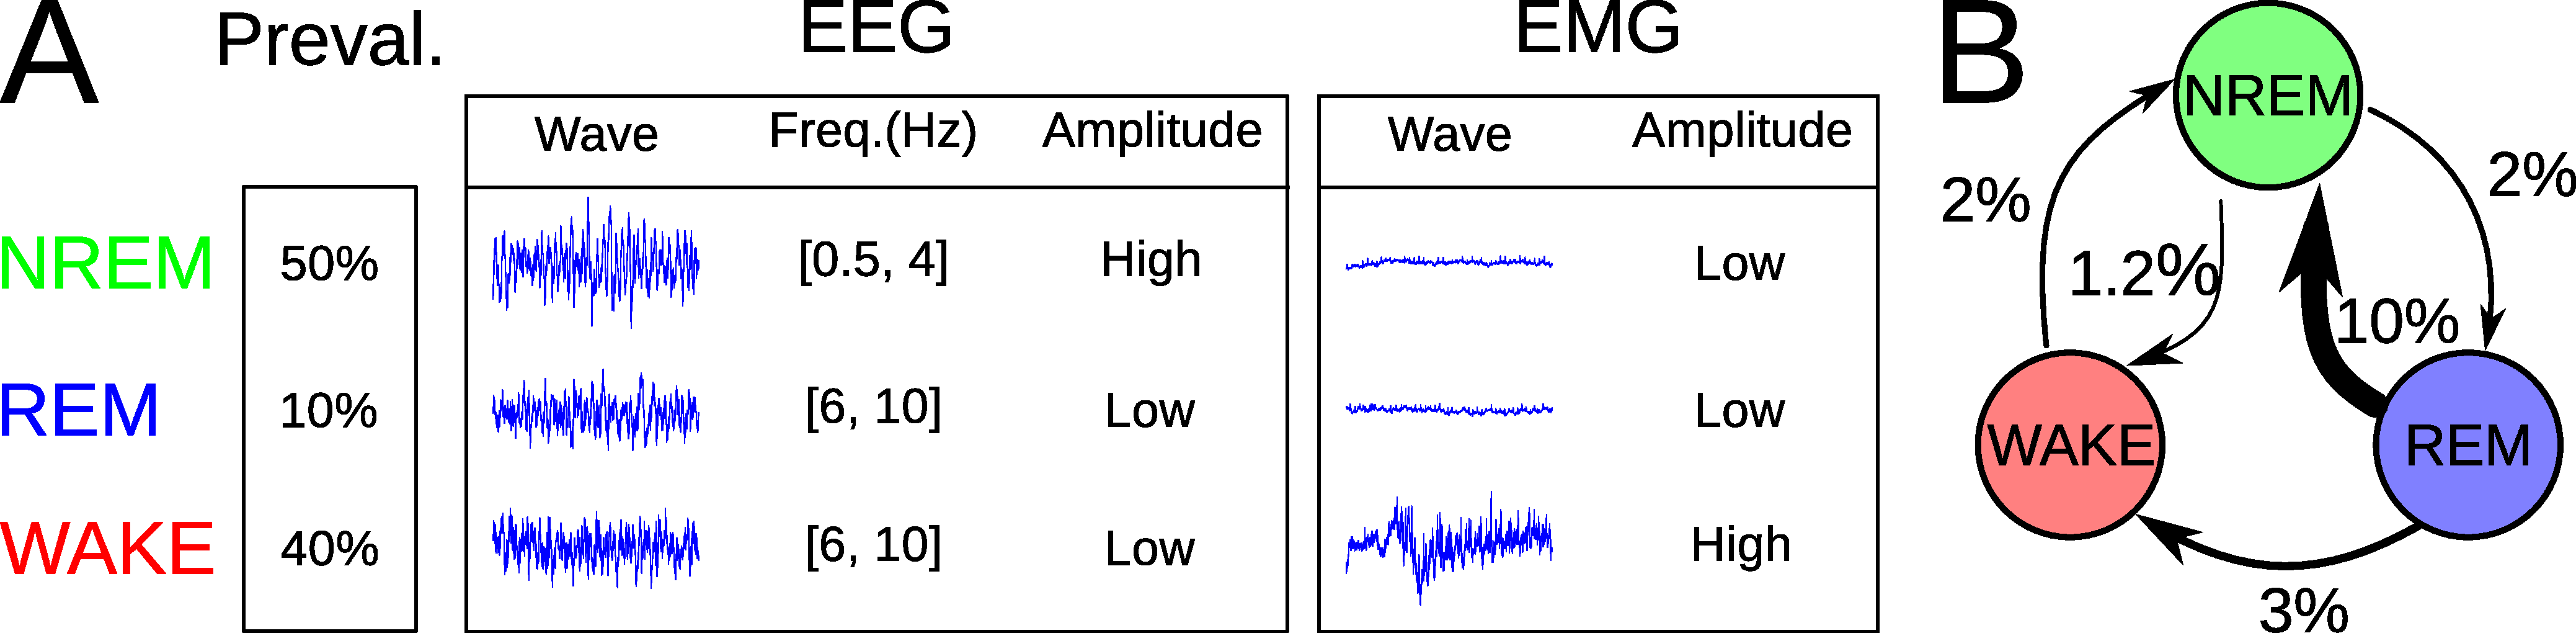
\includegraphics[width=0.95\textwidth]{figures/sleep_description.pdf}
  \caption{\ctit{Structural description of sleep stages.}
  \textbf{A}: Characteristics of the three sleep stages.
  Typically, frequency and amplitude of the \acrfull{eeg}, and amplitude of the \acrfull{emg} are used by experts to infer sleep stage.
  The presented frequency ranges and and pevalences are approximate values for healthy adult animals in normal conditions.
  Each wave shows a representative five second epoch with high signal to noise ratio.
  \textbf{B}: Empirical transition probabilities between consecutive five second epochs. The width of the arrow is proportionnal to the probability of transition.
  Probabilities of remaining in the three state are implied.
  \label{fig:sleep_description}
  }
           
\end{figure}



Although definitions of sleep stages appear straightforward, in practice, many cases are ambiguous.
For instance, it is difficult to characterise transitions between two states.
In addition, there are many sources of variability including how surgery was performed by the experimenter, the type of recorder used and inter-animal variability.
The quality of the acquisition can also be made considerably worst by noisy signals or by the presence of artefacts.
For these reasons, sleep scoring, the attribution of discrete vigilance states to electrophysiological time series,
is traditionally performed by trained human experts.
Such manual annotation is very time consuming; several hours of work have been reported in order to score 24h of recording.
This severely limits data throughput and human subjectivity is likely to introduce systematic bias.
Indeed, it is expected that scoring will be performed differently by each expert, making result difficult to reproduce independently.
Often, two experts score the same time data, in order to ensure satisfying agreement.
Although, manual scorers are generally reported as being very consensual\citationneeded{},
it can be argued that experts most likely work in the same laboratory and trained one another, or were trained by the same third person.
In this context, agreement between experts does not account for the variability between communities of researchers, and cannot be used to assess reproducibility.

In order to overcome both speed and subjectivity limitations, efforts have been directed towards automation of sleep scoring.
However, there is little adoption has occurred and very few available implementations in the form of software that biologists could use have been developed.
Typically, two different approaches to classification have been followed: unsupervised or supervised learning.

Unsupervised learning has the advantage of making no assumption about the nature of the different vigilance states, and how they should be defined.
Therefore, this approach can lead to the discovery of truly new states.
One issue is that the choice of the variables used for clustering is very critical.
Often, variables such as frequency domain variables are in fact chosen in order to generate clusters that will match human defined clusters.
In addition, unsupervised methods may lack robustness in so far as the cannot easily include covariates explaining, for instance, variability between recording equipments.

Another approach is to assume human annotations are, although imperfect, biologically relevant and generally consistent,
 and therefore to use supervised learning techniques.
Of course, if human decisions were biased, such a method may reproduce this bias.
However, a vast corpus of experimental work has provided hypothesis about function of these states which tends to validate the actual `existence' of these discrete vigilance states.
Building a classifier that would produce a consensual prediction of vigilance states could be seen as an attempt to formalised and rationalise the definition of such states.
This would improve future research without denying decades of sleep neurobiology.

Many supervised learning techniques ranging from SVM, ANNs, to HMMs have been investigated.
In general, the first step is to compute features on consecutive segments of annotated electrophysiological signals know as epochs.
Then, the relation between the response variable(annotation) and the independent variables (features) can be modelled.
Either epochs are considered to be independent from one another or time-dependent structures are explicitly modelled (\eg{} using HMMs).
Time aware modelling has the advantage of accounting for the interdependence of consecutive epochs (see fig.~\ref{fig:sleep_description}B).
However, it generally does not perform as well as classical classifiers when modelling non-linear relationships between large numbers of predictors.

Recently, promising results were obtained for scoring human sleep stages by performing an exhaustive
feature extraction including variables resulting from discrete wavelet decomposition.
Then, the authors compared several classifiers and found that random forest were, overall, the most accurate predictors.

The study herein bases itself on these promising results by computing an even larger number of features.
An important addition is the computation of time-aware features which significantly improved accuracy.
Furthermore, rigorous stratified cross-validation procedure and comparisons of sleep structure were performed.
These improvement altogether contributed to achieve a very satisfying overall accuracy of 92\%.
In order to pave the way to an implementation of an ubiquitous sleep scoring software.
\pr, a new \py{} package was also build to facilitate efficient feature extraction.
This new package is here demonstrated to be significantly more performance than alternative implementation.

